\documentclass[twocolumn, a4paper, 10pt]{article}
\usepackage[top=2cm, bottom=2.5cm, left=1.5cm, right=1.5cm]{geometry}
\usepackage{graphicx}
\usepackage{amsmath, amssymb, amsfonts}
\usepackage{booktabs}
\usepackage{float}
\usepackage{hyperref}
\usepackage{titlesec}
\usepackage{abstract}
\usepackage{enumitem}
\usepackage{fancyhdr}
\usepackage{tikz}
\usetikzlibrary{shapes.geometric, arrows, positioning, calc}

\titleformat{\section}{\large\bfseries}{\thesection}{1em}{}
\titleformat{\subsection}{\normalsize\bfseries}{\thesubsection}{1em}{}

\renewcommand{\abstractnamefont}{\large\bfseries}
\renewcommand{\abstracttextfont}{\normalfont}

\hypersetup{
    colorlinks=true,
    linkcolor=black,
    citecolor=blue,
    urlcolor=blue
}

\tikzstyle{process} = [rectangle, minimum width=2cm, minimum height=1cm, text centered, draw=black, fill=blue!5, font=\small]
\tikzstyle{decision} = [diamond, minimum width=1cm, minimum height=0.5cm, text centered, draw=black, fill=green!5, font=\small]
\tikzstyle{io} = [trapezium, trapezium left angle=70, trapezium right angle=110, minimum width=2cm, minimum height=1cm, text centered, draw=black, fill=orange!10, font=\small]
\tikzstyle{arrow} = [thick,->,>=stealth]

\title{\textbf{A Hybrid Feature-Engineering and LLM Framework for Social Role Prediction}\\ \large —— Kaggle Challenge: Influencer or Observer Solution Report}

\author{
    \textbf{Maroun Hindieh}, \textbf{Linh Vu Tu}, \textbf{Yuguang Yao} \\
    École Polytechnique \\
    \texttt{\{maroun.hindieh, linh-vu.tu, yuguang.yao\}@polytechnique.edu}
}

\date{December 2025}

\begin{document}

\maketitle

\begin{abstract}
\textbf{Abstract}：
Identifying influencers versus observers is key to understanding information diffusion. This work proposes a configurable, modular, robust, and auto-optimized framework for the Kaggle “Influencer or Observer” task. Given a Twitter dataset with 184 raw features (textual and non-textual metadata), we predict whether a user is an influencer or an observer. We combine deep feature engineering (construction and cleaning) to build robust tabular features, and fine-tune CamemBERT with a binary loss to extract penultimate-layer embeddings, then apply PCA to retain core semantics. Finally, we ensemble the Boosting family (XGBoost, CatBoost, LightGBM) on semantic and non-semantic features via weighted averaging, achieving a best Private LB score of \textbf{0.844}.

\vspace{0.5em}
\noindent \textbf{Keywords}：Kaggle, feature engineering, CamemBERT, PCA, Gradient Boosting, adversarial validation
\end{abstract}

\section{Introduction}

In modern digital ecosystems, distinguishing content producers (influencers) from consumers (observers) is crucial for advertising, public-opinion monitoring, and sociological studies. The challenge provides a mixed structured/unstructured dataset and asks for a single-tweet prediction of social role.

This is a binary classification problem with three main difficulties: (1) multi-modal heterogeneity between textual semantics and numerical statistics; (2) distribution shift between train and test; (3) highly nonlinear relations between tweet content and user behavior. We therefore design a modular pipeline (Figure \ref{fig:architecture}): raw tweets are first visualized and statistically profiled, then split into three branches (text, constructed, non-text features). Text is processed by a fine-tuned LLM (CamemBERT) with a 0/1 loss and PCA compression. Constructed and non-text features are engineered and fused with the reduced semantic features in a Boosting feature layer. Adversarial validation improves robustness before training the Boosting ensemble (XGBoost, LightGBM, CatBoost) with hyperparameter optimization, learning-curve monitoring, and n-fold CV. A weighted average produces final predictions. We also use SHAP for interpretability, forming a feedback loop from outputs to features. This paper details the end-to-end path from feature engineering and adversarial validation to LLM-based semantics and final ensembling.

\begin{figure*}[htbp]
\centering
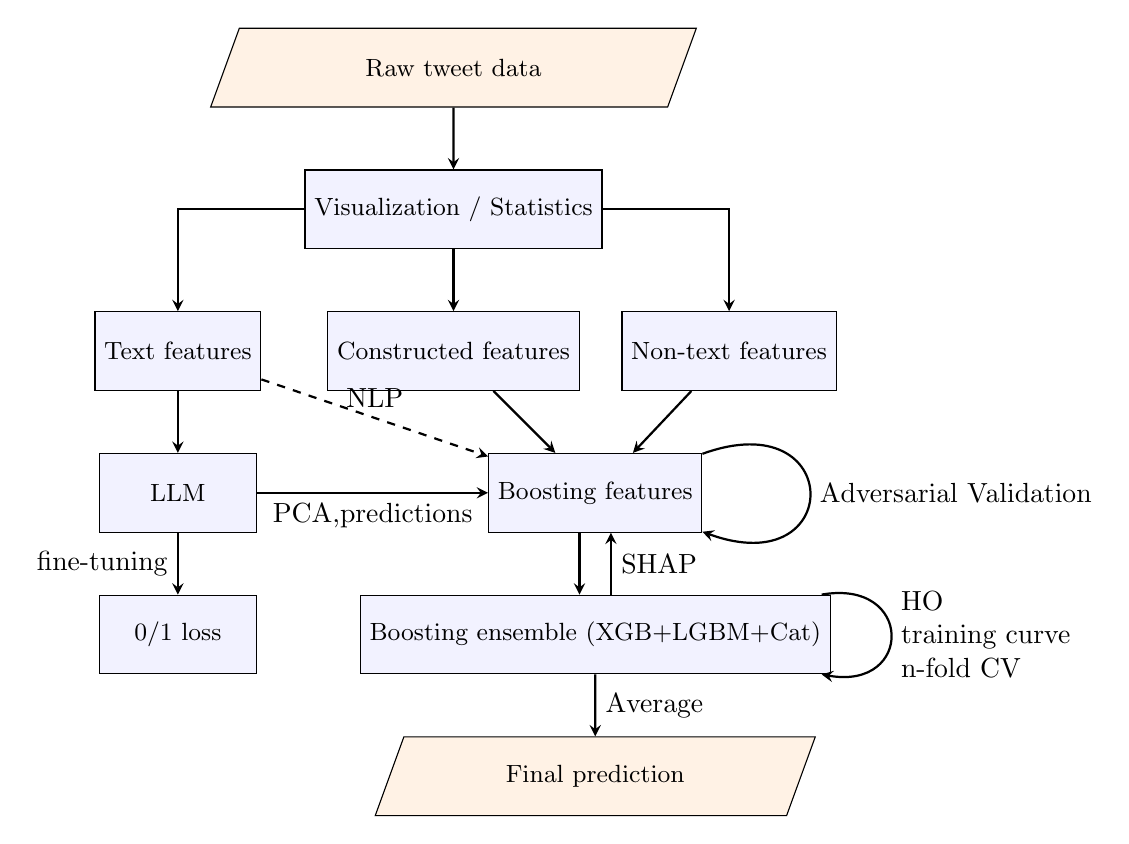
\begin{tikzpicture}[node distance=1.8cm]
    % Top: raw tweet data
    \node (input) [io] {Raw tweet data};
    
    % Fork: visualization/statistics
    \node (fork) [process, below of=input] {Visualization / Statistics};
    
    % Second layer: three feature branches
    \node (text) [process, below of=fork, xshift=-3.5cm] {Text features};
    \node (construct) [process, below of=fork] {Constructed features};
    \node (nontext) [process, below of=fork, xshift=3.5cm] {Non-text features};
    
    % Third layer: LLM and 0/1 loss
    \node (llm) [process, below of=text] {LLM};
    \node (loss) [process, below of=llm] {0/1 loss};
    
    % Fourth layer: Boosting feature fusion
    \node (boost_feature) [process, right of=llm, xshift=3.5cm] {Boosting features};
    
    \node (boost) [process, below of=boost_feature] {Boosting ensemble (XGB+LGBM+Cat)};
    % Fifth layer: final prediction
    \node (output) [io, below of=boost] {Final prediction};

    % From raw data to fork, then split to three feature nodes
    \draw [arrow] (input) -- (fork);
    \draw [arrow] (fork) -| (text);
    \draw [arrow] (fork) -- (construct);
    \draw [arrow] (fork) -| (nontext);
    
    % Text features -> LLM -> 0/1 loss
    \draw [arrow] (text) -- (llm);
    \draw [arrow] (llm) -- node[anchor=east] {fine-tuning} (loss);
    
    % LLM to boosting feature fusion (with PCA label)
    \draw [arrow] (llm) -- node[anchor=north] {PCA,predictions} (boost_feature);
    
    % Constructed and non-text features to boosting fusion
    \draw [arrow] (construct) -- (boost_feature);
    \draw [arrow] (nontext) -- (boost_feature);
    \draw [arrow, dashed] (text) -- node[anchor=south] {NLP} (boost_feature);
    
    % Boosting ensemble to final prediction
    % Arrow from boosting features to ensemble (slightly left)
    \draw [arrow] ([xshift=-0.2cm]boost_feature.south) -- ([xshift=-0.2cm]boost.north);
    \draw [arrow] (boost) -- node[anchor=west] {Average}(output);
    
    % Feedback loop from boosting ensemble to boosting features (SHAP)
    \draw [arrow] ([xshift=0.2cm]boost.north) -- node[anchor=west] {SHAP} ([xshift=0.2cm]boost_feature.south);
    
    % Self-loop on boosting features (Adversarial Validation)
    \draw [arrow] (boost_feature) to[out=20, in=340, looseness=5] node[anchor=west] {Adversarial Validation} (boost_feature);
    \draw [arrow] (boost) to[out=10, in=350, looseness=3] node[anchor=west, align=left] {HO\\training curve\\n-fold CV} (boost);
\end{tikzpicture}
\caption{Overall technical architecture: from adversarial feature filtering to multimodal feature fusion.}
\label{fig:architecture}
\end{figure*}

\section{Data Exploration and Feature Engineering}
\label{sec:feature_eng}

This section details the construction, cleaning, and filtering of non-text features (structured data and metadata). We ground decisions in EDA: dashboards in \texttt{output/visualizations} highlight heavy-tailed activity (\texttt{user.statuses\_count} median 7.3k vs. max 3.7M) and unstable ratios, motivating log transforms and per-day rates; text-length histograms (mean $\approx$107 chars, cap at 158) support the 256-token truncation; word-frequency plots dominated by URLs/mentions justify placeholder normalization; correlation heatmaps show low collinearity except for hashtag/mention/URL families, guiding a lean feature plan.

We convert these statistics into explicit rules: \texttt{feature\_statistics\_report.json} flags sparsity, leakage-prone IDs, and mutual-information strength for every column. The resulting recipes (drop, median-impute, frequency/target encode, etc.) are materialized in \texttt{src/preprocessing/feature\_processing\_plan.json} for explainability, while the main training pipeline applies the configuration in \texttt{setup.yml} to keep behavior reproducible and editable.

On this basis, we apply a configuration-driven, modular feature-engineering framework. During basic cleaning, numeric features are median-imputed, Booleans cast to integers, and categorical columns encoded via frequency or CV-based target encoding. Temporal signals parse timestamps into year/month/day/hour/weekday plus account age (no sine/cosine cyclical encoding); \texttt{statuses\_count} and \texttt{listed\_count} yield Tweets-per-Day and Listed-per-Day rates. The follower/following ratio is computed when both fields exist (not forcibly disabled).

For semi-structured metadata, regex-based extraction captures fine-grained user behavior. Parsing the HTML-formatted \texttt{source} reconstructs client type (mobile/web/pro tools/other). Text metadata adds length, mentions, hashtags, and URL flags; richer style cues such as repeated-character patterns \texttt{r'(.)\textbackslash 1\{2,\}'} are available in the CamemBERT style module but stay off by default unless \texttt{extract\_style\_features=true}.

To reduce leakage, IDs like \texttt{id} / \texttt{id\_str} are dropped via configuration; the plan also marks \texttt{timestamp\_ms} and train/test-shifted URL fields (e.g., \texttt{quoted\_status\_permalink.expanded}) for removal when the plan-driven preprocessing path is used. Remaining features are numeric and column-aligned, yielding a standardized matrix that balances stability and predictive power.



\section*{LLM-Based Semantic Feature Extraction}

To surpass the limits of shallow statistics (e.g., term frequency, length), we employ a pre-trained language model to derive high-dimensional tweet representations through multi-source fusion, model fine-tuning, and dimensionality reduction. In \textbf{input construction and preprocessing}, we fuse \texttt{extended\_tweet.full\_text}, \texttt{quoted\_status.text}, and \texttt{user.description} with separators such as \texttt{[SEP]} and \texttt{[USER\_DESC]}. HTML entities are unescaped; frequent URLs and media links are replaced by \texttt{<LINK\_URL>} and \texttt{<MEDIA\_URL>}; usernames become \texttt{@USER}, preserving structure while reducing noise.

In \textbf{model choice and fine-tuning}, we select \textbf{CamemBERT} as the core encoder. Text sequences are truncated to 256 tokens; the model is fine-tuned on the downstream task, and we extract the penultimate \texttt{[CLS]} vector or fine-tuned logits to obtain task-specific semantic representations.

For \textbf{feature reduction and fusion}, the 768-dimensional embeddings would otherwise create a curse-of-dimensionality risk for tree models. PCA compresses them to 16–32 orthogonal principal components, retaining key variance and balancing with non-text structured features to form a robust hybrid feature space.

\section*{Ensembling and Fusion Strategy}

We ensemble \textbf{XGBoost}, \textbf{LightGBM}, and \textbf{CatBoost} to improve robustness. A \textbf{5-fold stratified cross-validation} scheme trains on four folds and predicts the held-out fold, producing out-of-fold predictions that avoid leakage. To choose a fusion mechanism, we compute the \textbf{Pearson correlation coefficient} between base models. Predictions are highly correlated (0.97–0.99) and exhibit a notable \textbf{distribution shift} between train and test, so logistic-regression stacking overfits and degrades accuracy. We therefore adopt a shift-robust \textbf{rank-averaging} strategy: logits are converted to normalized ranks (0–1), reducing absolute-probability bias; weighted blending, with weights from CV AUC, yields the final stable prediction.

Beyond fixed defaults, each booster’s key hyperparameters (learning rate, depth, subsample, colsample, regularization) were tuned with Bayesian optimization (Optuna TPE) under 5-fold CV, favoring lower-variance configurations over marginal CV gains to curb overfitting. XGBoost runs on GPU (tree_method=hist, device=cuda) for faster exploration, while LightGBM/​CatBoost retain conservative depth and min-child settings. Final fusion remains rank-based and weight-calibrated by CV AUC, which proved more shift-tolerant than probability averaging or logistic stacking on these highly correlated base models.

\section*{Feature Validation and Model Explainability}

To detect distribution shift and leakage, we first apply \textbf{adversarial validation}. A binary XGBoost classifier separates train vs. test; its initial AUC above 0.99 exposed severe shift. Feature importance highlighted leakage and sampling-bias sources, notably \texttt{timestamp\_ms}, \texttt{id\_str}, \texttt{quoted\_status.id\_str}, \texttt{quoted\_status\_permalink.expanded}, and \texttt{is\_default\_background}. Removing these reduced adversarial AUC to 0.67, improving generalization safety.

We then use \textbf{SHapley Additive exPlanations (SHAP)} for decision analysis. Beeswarm plots show global influence (e.g., higher \texttt{listed\_per\_day} pushes toward “Influencer”); dependence plots reveal nonlinear interactions; waterfall plots explain individual cases. SHAP values also guide pruning: an adaptive threshold removes low-contribution features (mean absolute SHAP $<$ 0.001), reducing noise and improving robustness.

\section*{Explored but Not Adopted}

\textbf{DeBERTa-v3 with LoRA fine-tuning.} We trained \texttt{microsoft/deberta-v3-base} with optional LoRA adapters, focal loss, R-Drop, and gradient checkpointing to extract supervised [CLS] embeddings for downstream tree models. Despite Optuna tuning and 5-fold CV, the embeddings trailed CamemBERT by $\approx$0.01–0.015 AUC and required more GPU memory/time, so we kept it only as a fallback.

\textbf{Logistic stacking over boosters.} We tried a meta-classifier (logistic regression) on top of XGBoost/LightGBM/CatBoost OOF logits. High pairwise correlations (0.97–0.99) and train–test shift caused overfitting and worse public LB, while rank averaging stayed more stable. We therefore discarded the stacking variant and used rank-based fusion.

\section{Conclusion}

We built a configuration-driven multimodal feature-engineering framework that reconstructs client and text-style signals via regex and fuses CamemBERT semantic embeddings. To address severe distribution shift, we applied adversarial validation to remove leakage features (timestamps, IDs) and adopted rank averaging for more robust ensembling. Although performance is strong, adversarial validation shows residual shift and missing fields limit completeness. Future work should pursue deeper distribution alignment, fuller data cleaning, and end-to-end integration of large language models with tree-based learners to further improve generalization and accuracy.

\appendix




\end{document}